
\documentclass[11pt]{beamer}
\usetheme{CambridgeUS}

\usepackage[utf8]{inputenc}
\usepackage[english]{babel}
\usepackage{amsmath}
\usepackage{amsfonts}
\usepackage{amssymb}
\usepackage{graphicx}
\usepackage{subfigure}
\usepackage{algorithm2e}
\usepackage{algorithmic}
\usepackage{url}
\usepackage{float}



% Puts the right page numbers for the presentation
\setbeamertemplate{footline}[frame number]

% Show uncovered items: 0 is invisible, 100 is fully visible
\setbeamercovered{transparent=3}

\author{Cody, Venkatesh Jatla, Mustafa}
\title{Recommender systems}
\logo{
\includegraphics[width=2.5cm]{pictures/ecelogo.jpg}}
\institute{Dept of Electrical and Computer Engineering \\ The University of New Mexico \\ Albuquerque, NM 87131-0001, USA}
\date{April 8th, 2015}

\begin{document}
	\maketitle
	\section{Outline}
	\begin{frame}
		\frametitle{Outline}
		\begin{itemize}
			\item Collaborative filtering
			\begin{itemize}
				\item Data normalization
				\item Validation
				\item Algorithm
				\item Results
				\item References
			\end{itemize}
			\item Content based filtering
			\begin{itemize}
				\item Block diagram
			\end{itemize}
		\end{itemize}
	\end{frame}
	\section{Collaborative filtering}
	\begin{frame}
		\frametitle{Data normaliztaion}
		\begin{itemize}
			\item Input Data = \{user\_id, song\_id, plays\}
			\item Normalize {\bf plays} so that
			\begin{itemize}
				\item 10 $=>$ Most liked song
				\item 0 $=>$ Most disliked song
			\end{itemize}
			\item If user $u_x$ has $P = \{p_1. p_2, p_3,\dots,p_n	\}$, then
			\begin{equation}
				r_i = 10 \times p_i/max\{P\}
			\end{equation}
		\end{itemize}
	\end{frame}
	\begin{frame}
		\frametitle{Validation block diagram}
		\begin{figure}
		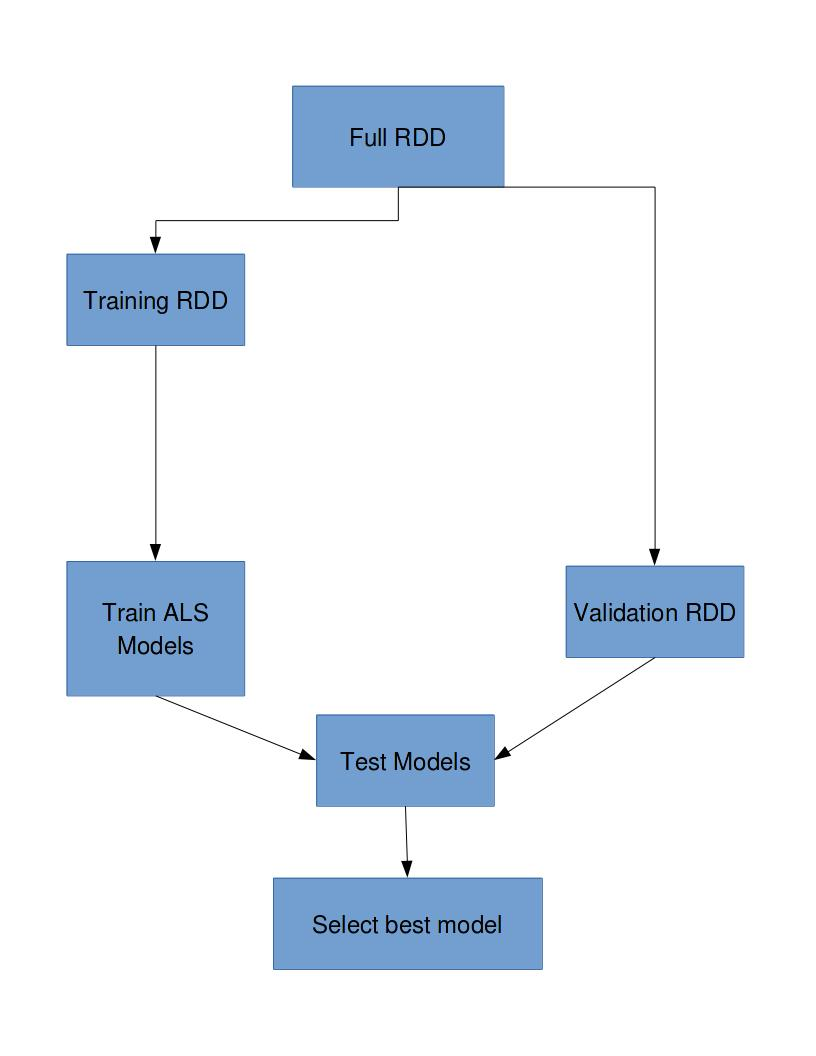
\includegraphics[width=0.5\linewidth]{pictures/Validation.jpg}
		\end{figure}
	\end{frame}
	\begin{frame}
		\frametitle{Validation}
		\begin{itemize}
			\item Free parameters in ALS, \href{'http://spark.apache.org/docs/latest/mllib-collaborative-filtering.html'}{tutorial}
				\begin{itemize}
					\item rank, $\{R_0,R_1,\dots\}$
					\item lambda, $\{L_0,L_1,\dots\}$
					\item numIters, $\{N_0,N1,\dots\}$
				\end{itemize}
			\item Let input data RDD be, $R = \{row_i\}$, $row_i = \{user\_id_i, song\_id_i, r_i\}$
			\item Validation RDD is created by {\bf randomly sampling 10\%} of data RDD, $VS = 0.1R$
			\item Training RDD is creted by {\bf intersection compliment} of data RDD and Validation RDD,
			$TS = R - (R \cap VS)$
			\item Every possible combination is iterated and the model that gives {\bf minimum RMSE} on
			validation set, $VS$ is picked as best model.
		\end{itemize}
	\end{frame}
	\begin{frame}
		\frametitle{Algorithm}
	\end{frame}
	\begin{frame}
		\frametitle{Results}
	\end{frame}
	\section{Content based filtering}
	\begin{frame}
		\frametitle{Block Diagram}
	\end{frame}

	\section{Test}
\end{document}
